\capitulo{3}{Conceptos teóricos}

Dentro de este proyecto existen elementos o implementaciones que pueden llegar a tener una mayor complejidad teórica. Por ese mismo motivo, en este apartado se van a detallar en diferentes secciones los aspectos más complejos que han surgido durante el desarrollo.

\section{Web scraping}
El \textit{web scraping}~\cite{Webscraping} es una técnica usualmente utilizada para poder obtener de forma automática y estructurada los contenidos de las páginas web para su utilización en diferentes fines. 
En el caso de este proyecto, para obtener los datos detallados de los libros deseados.

Esta técnica puede resultar muy beneficiosa debido a que se pueden obtener grandes volúmenes de datos minimizando las posibilidades de error frente a una búsqueda manual, la cuál es más lenta y costosa.

Aunque este sistema de obtención de datos sea muy útil y eficiente, antes de aplicarlo a una página web para la obtención de los datos, es imprescindible comprobar que esta página nos da la autorización para realizarlo.

Para realizar esta comprobación de manera legal y sencilla, y así evitar posibles problemas legales, es fundamental consultar el archivo \textit{robots.txt}~\cite{Robots.txt} de la página web. Este archivo es un protocolo de exclusión de robots que define a qué URLs de una página web pueden acceder los rastreadores o bots. Al acceder a la URL de la página web \textit{/robots.txt}, se puede verificar si la web permite o restringe el acceso a ciertos servicios y redireccionamientos para realizar \textit{web scraping}.

El archivo \textit{robots.txt} proporciona una lista de reglas que indican a los rastreadores web qué partes del sitio deben evitar, ayudando así a prevenir accesos no autorizados y proteger la integridad del sitio web. Este protocolo especifica, mediante directivas, qué áreas de la página web no deben ser rastreadas y puede incluir secciones como \textit{'Disallow'} para bloquear acceso a determinadas rutas o archivos y \textit{'Allow'} para permitir acceso a otras partes.

\begin{figure}[htbp]
    \centering
    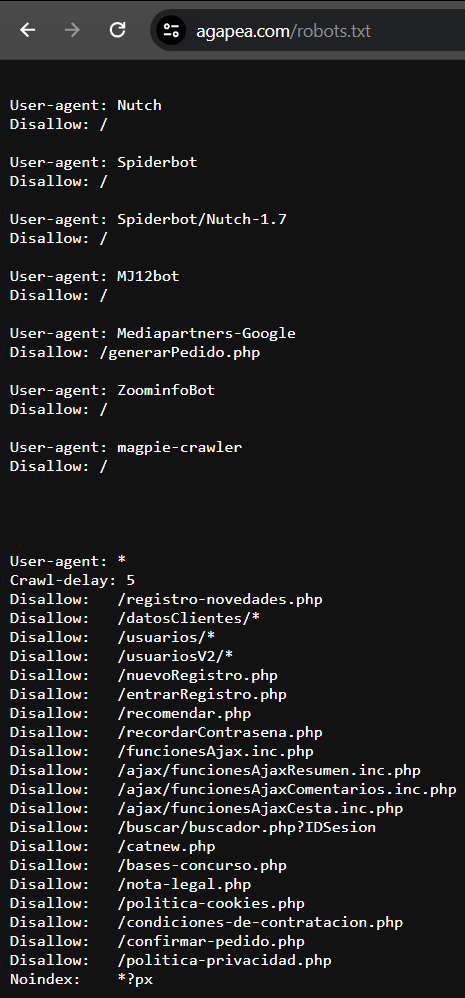
\includegraphics[width=0.5\linewidth]{Imagenes/RobotsAgapea.png}
    \caption{Archivo robots de Agapea}
    \label{Archivo robots de Agapea}
\end{figure}
\FloatBarrier
En la Figura \ref{Archivo robots de Agapea} podemos observar el archivo \textit{robots.txt} de la web de la librería Agapea \footnote{\href{https://www.agapea.com/robots.txt}{Enlace a robots.txt}}, la cual hemos utilizado en el desarrollo de este proyecto. Tal como se muestra, las primeras líneas hacen referencia a distintos rastreadores y servicios específicos los cuales no pueden acceder a las URL marcadas en el apartado de "disallow" (En este caso, los servicios que aparecen no tienen permisos para acceder a ninguna URL perteneciente a esta web).

Debajo de estas primeras líneas observamos otro grupo de líneas que son las que indican cuáles son las URL a las que no está permitida la entrada o utilización de ningún tipo de servicio o rastreador, indistintamente del tipo que sea.

Otras formas de bloqueo existentes que podrían afectar a la utilización de esta herramienta son las siguientes:
\begin{itemize}
    \item \textit{CAPTCHAs}:  Bloqueos simples para poder distinguir entre un robot y un humano.
    \item Limite de peticiones: Estableciendo un límite no se podrían obtener los datos de una forma tan rápida, ya que la propia web lo bloquea al superar el límite de peticiones.
    \item Bloqueo por IP: Las páginas web pueden contener una lista negra de usuarios que no puedan acceder a la web, esto se hace a través de listas de IPs.
\end{itemize}

Una vez se establecen las limitaciones y se tienen en cuenta en la aplicación del web scraping, se pueden utilizar diferentes herramientas para implementarlo, como bibliotecas o frameworks, que permiten un desarrollo correcto de análisis de los datos de las páginas web deseadas. En secciones posteriores se describen las utilizadas para este proyecto.


\section{Json Web Token (JWT)}
La tecnología JWT es una tecnología incluida en el estandar RFC 7519~\cite{JWT_Estandar} que permite enviar y recibir información de forma compacta y rápida dentro de un elemento JSON. Este elemento es muy seguro debido a que se encuentra firmado digitalmente.

\subsection{Estructura de un token JWT}
Para poder realizar las firmas y generar las claves, se suele utilizar una clave privada y única a partir de la cual se generan el resto, comúnmente utilizando el algoritmo SHA256.

En el caso de este proyecto, esta tecnología se ha utilizado para poder limitar el acceso a personas no autorizadas a los recursos de la API que han de ser privados y solo gestionados por aquellas personas que tengan la autorización pertinente.

Un token de acceso JWT tiene un patrón de construcción, ya que se divide en 3 partes separados por "." , los cuales se describirán a continuación~\cite{JWT_Info}.
\begin{itemize}
    \item Header
    \item Payload
    \item Signature
\end{itemize}

A continuación, se va a ir analizando un ejemplo de JWT, para ello utilizaremos un debugger de JWT~\cite{JWT_Debugger}:

Header:

\texttt{eyJhbGciOiJIUzI1NiIsInR5cCI6IkpXVCJ9}

En el header indica principalmente dos elementos, el tipo de algoritmo que se ha usado para generarlo, y que tipo de token es. En este caso se ha utilizado HS256.

\begin{figure}[htbp]
    \centering
    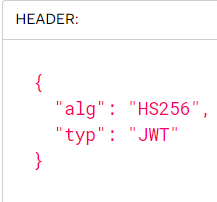
\includegraphics[width=0.5\linewidth]{Imagenes/HeaderJWT.png}
    \caption{Header}
    \label{Header}
\end{figure}
\FloatBarrier

Payload:

\texttt{eyJzdWIiOiIxMjM0NTY3ODkwIiwibmFtZSI6IkRhbmllbCBGZXJuw6FuZGV6IiwiaWF}

\texttt{0IjoxNTE2MjM5MDIyfQ}

El apartado del payload contiene informaciones como el nombre de usuario, la fecha de la creación del token, y a quiín se refiere el token.

\begin{figure}[htbp]
    \centering
    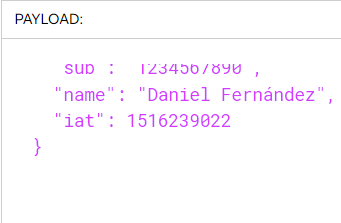
\includegraphics[width=0.5\linewidth]{Imagenes/JWT Payload.png}
    \caption{Payload}
    \label{Payload}
\end{figure}
\FloatBarrier

Signature:

\texttt{RrvHMGQTYf15y5\_WgdoH1HULZDRYukEmb5iMgAIwW0k}

Este último apartado es la firma del token, este apartado se forma con el algoritmo especificado en el apartado de \textit{header} junto con una clave secreta que se defina por el administrador y los apartados anteriores codificados.

\begin{figure}[htbp]
    \centering
    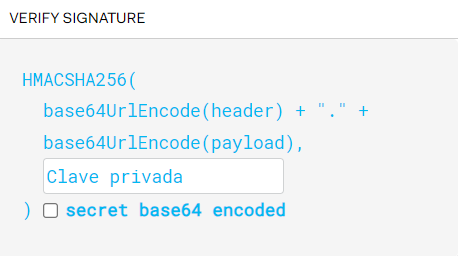
\includegraphics[width=0.5\linewidth]{Imagenes/JWTFirma.png}
    \caption{Signature}
    \label{Signature}
\end{figure}
\FloatBarrier

\subsection{Funcionamiento de un JWT }
Cada vez que una persona usuaria desea acceder a un recurso protegido con JWT, tiene que realizar una petición al \textit{backend} para que le retorne una clave nueva, si tenía una existente, no es necesario hacer la petición siempre y cuando ese token no expire.
En el caso de este proyecto, el token está configurado para proteger información de los usuarios registrados, además de no permitir la modificación ni obtención del catálogo. El token para poder realizar estas acciones se obtiene de manera invisible al usuario cuando realiza la operación de inicio de sesión.

Al obtener este token, es almacenado en el local storage del navegador, por lo que el usuario no necesita en ningún momento manipularlo ni editarlo.

Una vez obtenido, al realizar una petición al \textit{backend} será necesario incluir en la cabecera de la llamada el token generado. Esto se realiza internamente desde el \textit{frontend}, obteniendo el token de la zona de almacenamiento e incluyéndolo. Es importante mencionar que no siempre es necesario mandar al \textit{backend} el token, ya que en este proyecto no todas las llamadas lo requieren.

Tras este envío al servidor, el \textit{backend} realiza dos comprobaciones:
\begin{itemize}
    \item Fecha de expiración
    \item Validez del token
\end{itemize}
Si ambas comprobaciones resultan satisfactorias, el servidor responde a la petición correctamente.

\section{Estimación de la adecuación didáctica de los libros}
Este proyecto contiene un apartado que genera una estimación en un rango de 0 a 100 indicando al usuario la calidad de un libro introducido en términos de realidad científica en perspectiva de género. Este proceso de estimación se ha basado en la metodología publicada por Jesús Alberto San Martín Zapatero y Delfín Ortega Sánchez~\cite{san2022atribuciones}. Para realizar estos cálculos, el \textit{frontend} muestra al usuario un formulario donde tiene que rellenar los siguientes campos:
\begin{itemize}
    \item Campo de selección si existe masculino genérico.
    \item Cuatro campos donde se deben de introducir el número de personas adultas y menores existentes en el libro.
    \item Por cada uno de los géneros, se seleccionan las actividades que realizan de entre las opciones de una lista.
    \item La ubicación en la que se ambienta el libro.

\end{itemize}
Dentro de este formulario todos los campos son obligatorios exceptuando el de los menores, ya que es posible que no aparezcan, en cuyo caso la estimación se reajusta para adaptarse. Más detalles de la metodología de evaluación pueden encontrarse en ~\cite{san2022atribuciones}.

Una vez obtenidos estos datos se envían al \textit{backend} que va realizando las siguientes comprobaciones para ir ajustando la estimación.
\begin{enumerate}
    \item Obtiene el campo del masculino genérico y si la respuesta es negativa, se añaden 20 puntos a la nota final.
    \item En el caso de los contadores de personas, se realiza una media de equilibrio entre géneros tanto para personas adultas como para menores de forma independiente para obtener cómo de igualados están los dos géneros.  Idealmente tendrían que aparecer en la misma proporción o muy similar, lo que daría un resultado de 15 puntos para los personas adultas y 15 puntos para los menores. Si la proporción se encontrase desbalanceada, la nota sería menor ya sea en personas adultas o en menores.

En el caso de que el número total de menores existentes en el formulario sea el valor 0, la media se ajusta para no tener en cuenta este grupo y valorar sobre 30 puntos a los personas adultas.
\item Las actividades candidatas se encuentran contenidas en una tabla de la base de datos a las cuales los responsables de la administración pueden entrar y variar las actividades existentes y realizar una gestión completa. Por lo que, al llegar al \textit{backend}, los elementos seleccionados se cruzan con todos las actividades existentes y se obtienen de las comunes si le corresponde dar una puntuación extra o no por realizar esa acción (Una acción poco común para ese género, por lo tanto se premia). En base a estas comprobaciones se asignan hasta 20 puntos de la nota final de estimación.
\item Finalmente, el apartado de ubicaciones es un selector con unos valores fijos que se asignan y se envían en base a la elección del usuario. Cuanta más diversidad exista en la ubicación del libro, más cerca estará la puntuación de los 30 puntos de este apartado.

\end{enumerate}

Una vez terminado el análisis completo de los datos introducidos, se realiza una suma de todas las notas de cada apartado y se envía en escala 0-100, donde 0 es un libro muy poco adecuado y 100 es un libro que se corresponde a la perfección con la evidencia científica. Tras esto, el \textit{frontend} muestra al usuario un botón donde puede registrar su respuestas para que posteriormente los personas colaboradoras y responsables de la administración de la web puedan analizarlo y considerar agregar ese libro de cuya estimación ha sido realizada.




